\anonsection{Задание 9}
\anonsubsection{Формулировка задания}
Рассмотреть два вида процессов:
\begin{itemize}
	\item Винеровский процесс \( W(t), t\in[0,1], W(0) = 0 \).
	
	\item Процесс Орнштейна--Уленбека \( X(t), t\in[0,1], X(0) = X_0 \), 
     то есть стационарный марковский гауссовский процесс. Начальные 
     значения \( X_0 \) генеруются случайным образом так, чтобы полученный 
     процесс был стационарным.
	
\end{itemize}

Для данных гауссовских процессов
\begin{enumerate}
	\item Найти ковариационную функцию и переходные вероятности.
	
	\item Моделировать независимые траектории процесса с данными 
     переходными вероятностями методом добавления разбиения отрезка.
	
	\item Построить график траектории, не соединяя точки ломаной, с целью 
     получения визуально непрерывной линии.
\end{enumerate}

 
\anonsubsection{Винеровский процесс}

\begin{definition}
	Пусть дано вероятностное пространство \( (\Omega,\mathcal{F}, 
    \mathbb{P}) \). Параметризованное семейство \( \lbrace W_t\rbrace_{t \in 
     T} \) случайных величин
	\[
	 W_t(\cdot): \Omega \to \mathbb{R}, \quad t \in T,
	\]
	где \( T \subset[0, +\infty) \) интерпретируется как временной интервал, 
     называется случайным процессом.
\end{definition}
\begin{definition}
	Пусть дан случайный процесс \( \lbrace W_t \rbrace_{t\in T} \). Тогда 
     он называется гауссовским, если для любых \( t_0,t_1, \dots, t_n \in T \) 
     случайный вектор \( (W_{t_1}, W_{t_2}, \dots, W_{t_n}) \) имеет 
     многомерное нормальное распределение.
\end{definition}

Определим винеровский процесс как гауссовский процесс в отрезке 
 \( [0,1] \) со средним \( 0 \) и ковариационной функцией \( \text{cov} 
 \left(W(t_i), W(t_j) \right) = \min \left( t_i, t_j \right) \).

Основные свойства винеровского процесса:
\begin{itemize}
	\item $W_0=0$ почти наверное;
	\item $W_t$ является непрерывной функцией от $t$;
	\item Приращения функции $W(t)$ независимы и имеют нормальное 
     распределение со средним равным 0: $W_t - W_s \sim \mathcal{N} (0,1), 
     \quad s < t $.
\end{itemize}
Определим плотность $n$-мерного нормального распределения с невырожденной 
 ковариационной матрицей.
\begin{definition}
	Пусть $x$ --- $n$-мерный вектор и $ x \sim \mathcal{N}(m_x, R_x) $. 
     Тогда его плотность имеет вид
	\[
	 p(x) = \dfrac{1}{(2\pi)^{\frac{n}{2}}\sqrt{|R_x|}}e^ {-\frac{1}{2}
     (x-m_x)^T R_x^{-1}(x-m_x)},
	\]
	где $R_x$ --- ковариационная матрица.
\end{definition}
Смоделируем винеровский процесс методом деления отрезка $[0,1]$, в 
 отношении $\alpha$, исходя из следующих соображений:
\begin{enumerate}
	\item В начальный момент времени $W_{t_0}=0$, по определению;
	\item Генерируем $W_{t_1}=W_{t_1}-W_{t_0}\sim\mathcal{N}(0,1)$;
	\item Рассмотрим отрезок $[t_1,t_2]$, его внутреннюю точку $t = t_1 + 
     \alpha(t_2 - t_1)$ и условную плотность
	\begin{equation}\label{dens}
	    p_{W_t}(x \mid W_{t_1} = x_1, W_{t_2} = x_2) = \dfrac{p_{W_{t_1}, 
         W_t, W_{t_2}}(x_1, x, x_2)}{p_{W_{t_1}, W_{t_2}}(x_1, x_2)}. 
	\end{equation}
	 Обозначим векторы $ \bar{x} = (x_1, x, x_2)^T $ и $ \hat{x} = (x_1, 
     x_2)^T $ и рассмотрим плотности вероятностей этих векторов:
	$$
	\begin{aligned}
	    p_{W_{t_1}, W_t, W_{t_2}} & = \dfrac{1}{(2 \pi)^{\frac{3}{2}} 
         \sqrt{|R_1|}} e^{-\frac{1}{2} \bar{x}^T R_1^{-1} \bar{x}},\\
	    p_{W_{t_1}, W_{t_2}} &= \dfrac{1}{(2 \pi) \sqrt{|R_2|}} 
         e^{-\frac{1}{2}\hat{x}^T R_2^{-1} \hat{x}},
	\end{aligned}
	$$
	где $R_1,R_2$ --- соответствующие матрицы ковариаций. Так как 
     ковариационная функция имеет вид $k(s,t) = \min(s,t)$, то находим 
     выражения для $R_1$ и $R_2$:
	$$
	\begin{aligned}
	    & R_1 = \begin{pmatrix}
	        t_1 & t_1 & t_1 \\
	        t_1 & t & t \\
	        t_1 & t & t_2
	    \end{pmatrix} ,\\
	    & R_2 = \begin{pmatrix}
	        t_1 & t_1 \\
	        t_1 & t_2
	    \end{pmatrix}.
	\end{aligned}
	$$
	Вычислим определители и обратные матрицы для $R_1$ и $R_2$:
	\begin{gather*}
	|R_1|=t_1(t-t_1)(t_2-t), \\
	R_1^{-1}=\begin{pmatrix}
	\dfrac{t}{t_1(t-t_1)} & -\dfrac{1}{t-t_1} & 0 \\
	-\dfrac{1}{t-t_1} & \dfrac{t_2-t_1}{(t_2-t)(t-t_1} & -\dfrac{1}{t_2-t} \\
	0 & -\dfrac{1}{t_2-t} & \dfrac{1}{t_2-t}
	\end{pmatrix}, \\
	|R_2|=t_1(t_2-t_1), \\
	R_2^{-1}=\begin{pmatrix}
	\dfrac{t_2}{t_1(t_2-t_1)} & -\dfrac{1}{t_2-t_1} \\
	-\dfrac{1}{t_2-t_1} & \dfrac{1}{t_2-t_1}
	\end{pmatrix}.
	\end{gather*}
	В итоге получим:
	\begin{equation}\label{pW}
	    p_{W_t}(\,x \mid W_{t_1} = x_1, W_{t_2} = x_2\,) = \dfrac{1}{\sqrt{2 
         \pi \alpha (1 - \alpha)(t_2 - t_1)}} e^{-\dfrac{\left(x - ((1 - \alpha)
         x_1 + \alpha x_2) \right)^2}{2 \alpha(1 - \alpha)(t_2-t_1)}}. 
	\end{equation}
\end{enumerate}
Приведем итоговый алгоритм построения. 
\begin{enumerate}
	\item $t_0 = 0,\ t_1=1,\ W_{t_0}=0$, разыгрываем $W_{t_1} \sim 
     \mathcal{N}(0,1)$;
	\item Рекурсивно делим отрезки $[t_0,t_1],\ [t_0,t],\ [t,t_1]$ и т.~д. 
     в отношении $ \alpha $ к $ 1 - \alpha $ и разыгрываем случайные 
     величины $W_t$ с условной плотностью \eqref{pW} (то есть имеющие 
     нормальное распределение с математическим ожиданием $(1 - \alpha) 
     x_1 + \alpha x_2 $ и дисперсией $ \alpha(1 - \alpha)(t_2 - t_1)$) до 
     тех пор, пока не достигнем заданной точночти $t_{k + 1} - t_k < \epsilon$.
\end{enumerate}

\anonsubsection{Процесс Орнштейна--Уленбека}

\begin{definition}
	Случайный процесс \( \lbrace W_t\rbrace_{t\in T} \) называется 
     стационарным, если конечномерные распределения инвариантны 
     относительно сдвига времени.
\end{definition}

\begin{definition}
	Гауссовский процесс \( \lbrace W_t\rbrace_{t\in T} \) называется 
     процессом Орнштейна--Уленбека, если он является стационарным и 
     марковским.
\end{definition}

Из стационарности процесса Орнштейна--Уленбека следует, что
\[
\mathbb{E}W_t=a,\quad R(t,s)=R(|s-t|).
\]

Без ограничения общности положим \( a=0 \).

Обозначим \( \mathbb{D}W_t=\sigma^2 \), тогда \( R(t,s) \) представима в 
 виде \( R(t,s)=\sigma^2\rho(s,t) \), где \( \rho(s,t) \)~---~коэффициент 
 корреляции.

\begin{theorem}\footnote{Доказательство представлено в \cite{prob_feller}.}
	Для того чтобы последовательность \( W_1,\ldots,W_n \) нормально 
     распределённых случайных величин была марковской, необходимо и 
     достаточно, чтобы
	\[
	\rho_{j,k} = \rho_{j,i} \rho_{i,k} \ \forall i,j,k: j \leq i < k \leq n,
	\]
	где \( \rho_{i,j} \)~---~коэффициент корреляции случайных величин 
     \( W_i \) и \( W_j \).
\end{theorem}

В силу того, что процесс \( W_t \) является марковским, получаем, что
\begin{equation} \label{mark}
\rho(s,t)=\rho(s,\tau)\rho(\tau,t).
\end{equation}

Поскольку \( R(s,t)=R(|s-t|) \), то \( \rho(s,t)=\rho(s-t) \). Тогда, введя замену
\[
x=s-\tau,
\]
\[
y=\tau-t,
\]
преобразуем выражение~(\ref{mark}) к выражению
\[
\rho(x+y)=\rho(x)\rho(y).
\]

\begin{theorem}\footnote{Доказательство представлено в \cite{prob_feller}.}
	Пусть функция \( u(t) \) определена при \( t>0 \) и ограничена на 
     каждом конечном интервале. Если \( u(t) \) удовлетворяет соотношению 
     \( u(t+s)=u(t)u(s) \), то или \( u(t)\equiv0 \), или \( u(t) = 
     e^{-\lambda t} \), где \( \lambda \)~---~некоторая положительная 
     константа.
\end{theorem}

Если \( \rho(t) \equiv 0 \), то \( \text{cov}(W_t,W_s)=0 \), что 
 равносильно тому, что \( W_t \) независимы в совокупности (так как 
 процесс является гауссовским), поэтому поделирование процесса 
 Орнштейна--Уленбека заключается в моделировании случайных величин, 
 имеющих распределение \( N(a,\sigma^2) \).

Рассмотрим теперь случай \( \rho(s,t)=e^{-\lambda|s-t|} \), \( \lambda>0 \). 
 Ковариационная функция процесса Орнштейна--Уленбека имеет вид
\[
R(s,t)=\sigma^2e^{-\lambda|s-t|}.
\]

Найдём переходную плотность
\[
p_{W_t}(x_1|W_s=x_2)=\dfrac{p_{W_t,W_s}(x_1,x_2)}{p_{W_s}(x_2)}.
\]

Поскольку \( W_t \)~---~гауссовский процесс, то
\[
p_{W_t,W_s}(x_1,x_2)=\dfrac{1}{2\pi|C|^{\frac{1}{2}}}\exp\left\lbrace - 
 \dfrac{1}{2}(x,C^{-1}x)\right\rbrace,
\]
\[
p_{W_s}(x_2)=\dfrac{1}{\sqrt{2\pi}\sigma}\exp\left\lbrace - \dfrac{x_2^2}
 {2\sigma^2}\right\rbrace,
\]
где \( x=(x_1,x_2) \). Ковариационная матрица \( C \) имеет вид
\[
C=\begin{pmatrix}
\sigma^2&R(t,s)\\
R(t,s)&\sigma^2
\end{pmatrix}.
\]

Тогда
\[
|C|=\sigma^4-R^2(t,s), C^{-1}=\dfrac{1}{|C|}\begin{pmatrix}
\sigma^2&-R(t,s)\\
-R(t,s)&\sigma^2
\end{pmatrix}.
\]

Поэтому
\[
p_{W_t}(x_1|W_s=x_2)=\dfrac{1}{\left(2\pi\left(\sigma^2-\dfrac{R^2(t,s)}
 {\sigma^2}\right)\right)^{\frac{1}{2}}}\exp\left\lbrace-\dfrac{\left(x_1 - 
 \dfrac{R(t,s)}{\sigma^2}x_2\right)^2}{2\left(\sigma^2-\dfrac{R^2(t,s)}
 {\sigma^2}\right)}\right\rbrace,
\]
то есть
\[
F(W_t|W_s=x_2)\sim N\left(x_2e^{-\lambda|t-s|},\sigma^2\left(1-e^{-2 
 \lambda|t-s|}\right)\right).
\]

Так как рассматриваемый процесс является марковским, то, зная случайные 
 величины \( W_{t_1} \), \( W_{t_2} \), мы можем сгенерировать случайную 
 величину \( W_t \), где \( t_1<t<t_2 \). Будем моделировать \( W_t \) 
 аналогично моделированию винеровского процесса. Для упрощения положим 
 \( \alpha=1/2 \). Найдём условную плотность
\[
p_{W_{t}}(x|W_{t_1}=x_1,W_{t_2}=x_2)=\dfrac{p_{W_{t_1}W_tW_{t_2}}(x_1, x, 
 x_2)}{p_{W_{t_1},W_{t_2}}(x_1,x_2)},
\]
где \( t = (t_1 + t_2)/2 \). Поскольку процесс \( W_t \) является 
 гауссовским, то
\[
p_{W_{t_1}W_tW_{t_2}}(x_1,x,x_2) = \dfrac{1}{\left( 2 \pi \right)^{\frac{3}
 {2}} \left| R_1 \right|^{\frac{1}{2}}}\exp\left\lbrace-\dfrac{1}{2}(x_1, 
 x, x_2)^TR_1^{-1}(x_1,x,x_2)\right\rbrace,
\]
\[
p_{W_{t_1}W_{t_2}}(x_1,x_2)=\dfrac{1}{2\pi\left|R_2\right|^{\frac{1}{2}}} 
 \exp\left\lbrace-\dfrac{1}{2}(x_1,x_2)^TR_2(x_1,x_2)\right\rbrace,
\]
где
\[
R_1=\sigma^2\begin{pmatrix}
1&e^{-\lambda(t-t_1)}&e^{-\lambda(t_2-t_1)}\\
e^{-\lambda(t-t_1)}&1&e^{-\lambda(t_2-t)}\\
e^{-\lambda(t_2-t_1)}&e^{-\lambda(t_2-t)}&1
\end{pmatrix},\quad
R_2=\sigma^2\begin{pmatrix}
1&e^{-\lambda(t_2-t_1)}\\
e^{-\lambda(t_2-t_1)}&1
\end{pmatrix}.
\]

После ряда преобразований получим
\[
W_t\sim N\left((x_1+x_2)\dfrac{e^{-\frac{\lambda(t_2-t_1)}{2}}}{1 + 
 e^{-\lambda(t_2-t_1)}},\sigma^2\dfrac{1-e^{-\lambda(t_2-t_1)}}{1 + 
 e^{-\lambda(t_2-t_1)}}\right).
\]

В качестве \( W_0 \) и \( W_1 \) возьмём
\[
W_0\sim N(0,\sigma^2),W_1\sim N\left(x_0e^{-\lambda T}, \sigma^2\left(1 - 
 e^{-2\lambda T}\right)\right).
\]

\begin{figure}[ht]
    \centering
    \begin{subfigure}[b]{0.49\textwidth}
        \centering
        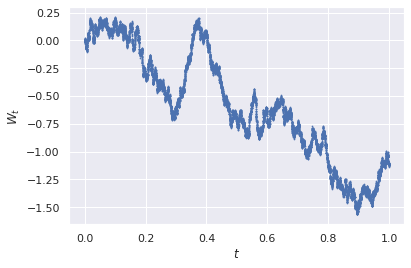
\includegraphics[width=\textwidth]{./resources/wiener_process.png}
        \caption{Винеровский процесс на отрезке $ [0, 1] $.}
        \label{subfig:wiener}
    \end{subfigure}
    \hfill
    \begin{subfigure}[b]{0.49\textwidth}
        \centering
        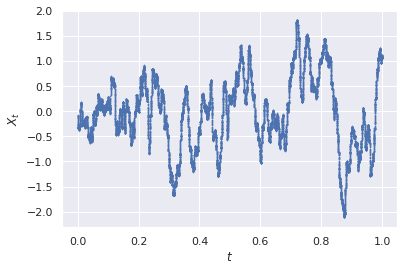
\includegraphics[width=\textwidth]{./resources/Orn_Uhl_process.png}
        \caption{Процесс Орнштейна-Уленбека на отрезке $ [0, 1] $.}
        \label{subfig:Orn_Uhl}
    \end{subfigure}
    \caption{Графики смоделированных процессов.}
    \label{fig:processes}
\end{figure}